\section{Futures} \label{futures}
Consider the parallel arrow combinator in Fig.~\ref{fig:someCombinator}
\begin{figure}[h]
\begin{lstlisting}[frame=htrbl]
someCombinator :: (Arrow arr) => [arr a b] -> [arr b c] -> arr [a] [c]
someCombinator fs1 fs2 = parEvalN () fs1 >>> rightRotate >>> parEvalN () fs2
\end{lstlisting}
\caption{An example parallel Arrow combinator without Futures}
\label{fig:someCombinator}
\end{figure}
In a distributed environment, the resulting arrow of this combinator first evaluates all \code{[arr a b]} in parallel, sends the results back to the master node, rotates the input once and then evaluates the \code{[arr b c]} in parallel to then gather the input once again on the master node. 
Such situations arise, \eg in scientific computations when the data distributed across the nodes needs to be transposed. A concrete example is 2D FFT computation \cite{Gorlatch,Berthold2009-fft}.

While the example in Fig.~\ref{fig:someCombinator} could be rewritten into only one \code{parEvalN} call by directly wiring the arrows properly together, this example illustrates an important problem: When using a \code{ArrowParallel} backend that resides on multiple computers, all communication between the nodes is done via the master node, as shown in the Eden trace in Figure~\ref{fig:withoutFutures}. This can become a serious bottleneck %in heavy threaded applications.
for larger amount of data and number of processes \citep[showcases][as, \eg]{Berthold2009-fft}.
\begin{figure}[ht]
	\centering
	\includegraphics[width=0.9\textwidth]{images/withoutFutures}
	\caption[without Futures]{Communication between 4 threads without Futures. All communication goes through the master node. Each bar represents one process. Black lines between processes represent communication. Colors: blue $\hat{=}$ idle, green $\hat{=}$ running, red  $\hat{=}$ blocked, yellow $\hat{=}$ suspended.}
	\label{fig:withoutFutures}
\end{figure}

This motivates for an approach that allows the nodes to communicate directly with each other. Thankfully, Eden, the distributed parallel Haskell we have used in this paper so far, already ships with the concept of \code{RD} (remote data) that enables this behaviour \cite{AlGo03a,Dieterle2010}.

But as we want code written against our API to be implementation agnostic, we have to wrap this context. We do this with the \code{Future} typeclass (Fig.~\ref{fig:future}).
\begin{figure}[h]
\begin{lstlisting}[frame=htrbl]
class Future fut a | a -> fut where
    put :: (Arrow arr) => arr a (fut a)
    get :: (Arrow arr) => arr (fut a) a
\end{lstlisting}
\caption{Definition of the Future typeclass}
\label{fig:future}
\end{figure}
Since \code{RD} is only a type synonym for communication type that Eden uses internally, we have to use some wrapper classes to fit that definition, though, as seen in Fig.~\ref{fig:RDFuture} (this is due to the same reason we had to introduce a wrapper for \code{Strategy a} in the Multicore Haskell implementation of \code{ArrowParallel} in chapter \ref{sec:parrows:multicore}).
\begin{figure}[h]
\begin{lstlisting}[frame=htrbl]
data RemoteData a = RD { rd :: RD a }

instance (Trans a) => Future RemoteData a where
    put = arr (\a -> RD { rd = release a })
    get = arr rd >>> arr fetch
\end{lstlisting}
\caption{RD based RemoteData version of Future for the Eden backend}
\label{fig:RDFuture}
\end{figure}

For our Par Monad and Multicore Haskell backends, we can simply use \code{MVar}s \cite{jones1996concurrent} (Fig.~\ref{fig:MVarFuture}), because we have shared memory in a single node and don't require Eden's sophisticated communication channels. \fixme{explain MVars}
\begin{figure}[h]
\begin{lstlisting}[frame=htrbl]
{-# NOINLINE putUnsafe #-}
putUnsafe :: a -> MVar a
putUnsafe a = unsafePerformIO $ do
    mVar <- newEmptyMVar
    putMVar mVar a
    return mVar

instance (NFData a) => Future MVar a where
    put = arr putUnsafe
    get = arr takeMVar >>> arr unsafePerformIO
\end{lstlisting}
\caption{MVar instance of the Future typeclass for the Par Monad and Multicore Haskell backends}
\label{fig:MVarFuture}
\end{figure}

Furthermore, in order for these \code{Future} types to fit with the \code{ArrowParallel} instances we gave earlier, we have to give the necessary \code{NFData} and \code{Trans} instances - the latter only being needed in Eden. Because \code{MVar} already ships with a \code{NFData} instance, we only have to supply two simple instances for our \code{RemoteData} type.
\begin{figure}[h]
\begin{lstlisting}[frame=htrbl]
instance NFData (RemoteData a) where
    rnf = rnf . rd
instance Trans (RemoteData a)
\end{lstlisting}
\caption{NFData and Trans instances for the RemoteData type. The Trans instance does not have any functions declared as the default implementation suffices here. See \url{https://hackage.haskell.org/package/edenmodules-1.2.0.0/docs/Control-Parallel-Eden.html\#g:5} for more information.}
\end{figure}
\\\\
Going back to our communication example we can use this Future concept in order to enable direct communications between the nodes in the following way:
\begin{lstlisting}[frame=htrbl]
someCombinator :: (Arrow arr) => [arr a b] -> [arr b c] -> arr [a] [c]
someCombinator fs1 fs2 =
	parEvalN () (map (>>> put) fs1) >>>
	rightRotate >>>
	parEvalN () (map (get >>>) fs2)
\end{lstlisting}
In a distributed environment, this gives us a communication scheme with messages going through the master node only if it is needed - similar to what is shown in the trace in Fig.~\ref{fig:withFutures}.\olcomment{Fig.~3 is not really clear. Do Figs 2-3 with a lot of load?}
\begin{figure}[ht]
	\centering
	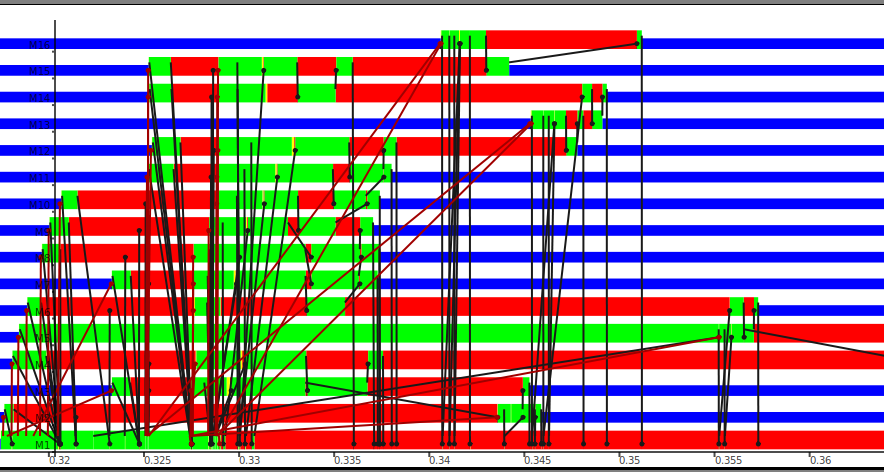
\includegraphics[width=0.9\textwidth]{images/withFutures}
	\caption[with Futures]{Communication between 4 threads with Futures. Other than in Fig.~\ref{fig:withoutFutures}, threads communicate directly (black lines between the bars) instead of always going through the master node (bottom bar).}
	\label{fig:withFutures}
\end{figure}